ue1:

1.Aufgabe:
\begin{equation}
\begin{split}
b \in \left\{ x_1 \cdot \begin{pmatrix*} 1\\ 1\\ 1 \end{pmatrix*} + x_2 \cdot \begin{pmatrix*} 1\\ -2\\ -1 \end{pmatrix*} | x_1, x_2 \in \R \right\}
\end{split}
\end{equation}
eine möglichst \glqq gute\grqq{} Lösung könnte sinnvollerweise foglendes erfüllen:

\[
\norm{Ax-b}^2_2 \longrightarrow min
\]

2.Aufgabe:
\begin{figure}[ht]
	\centering
	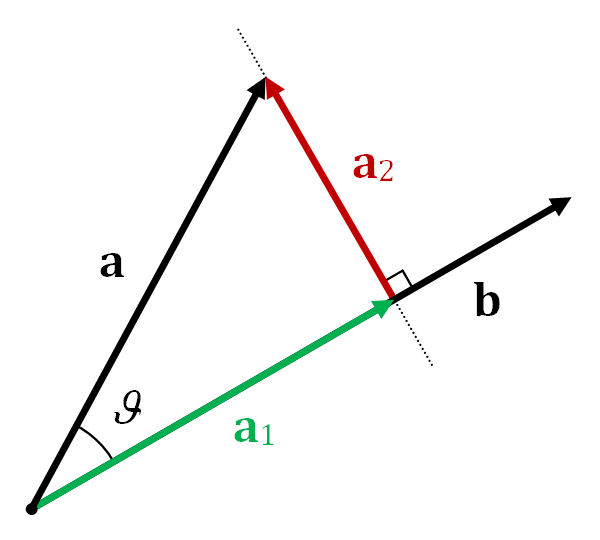
\includegraphics[scale=.3]{Projection_and_rejection.png}
\end{figure}

\begin{equation}\begin{split}
	u = \begin{pmatrix*}1\\1\\1\end{pmatrix*}\quad;\quad
	v = \begin{pmatrix*}0\\2\\1\end{pmatrix*}\\
	v = v_{\bot} + v_{\parallel}\\\\
\end{split}\end{equation}
\begin{equation}\begin{split}
	<v; u>
	&= <v_{\bot} + v_{\parallel}; u>\\
	&= <v_{\bot}; u> + <v_{\parallel}; u>\\
	&= \cancelto{0}{<v_{\bot}; u>} \quad + <v_{\parallel}; u>\\
	&= <v_{\parallel}; u>\\
\end{split}\end{equation}

\begin{equation}\begin{split}
	v_u = \begin{pmatrix*}1\\1\\1\end{pmatrix*}
\end{split}\end{equation}
\begin{equation}\begin{split}
	u_v = \begin{pmatrix*}-1\\1\\0\end{pmatrix*}
\end{split}\end{equation}

Orthogonale Projektion:
\begin{equation}\begin{split}
	u \rightarrow P_u : v &\mapsto v_1\\
	v &\mapsto P_u(v) = \frac{<v;u>}{<u;u>} u = \frac{1}{<u;u>} u \cdot u^T v
\end{split}\end{equation}
\begin{equation}\begin{split}
	v &\mapsto \frac{1}{\norm{u}^2}u^T v \cdot u = y\\
	y_i &= \frac{1}{\norm{u}^2}u_i(u_1v_1 + u_2v_2 + u_3v_3)\\
	&\stackrel{!}{=} a_{i1}v_1 + a_{i2}v_2 + a_{i3}v_3\\
	a_{ij} &= \frac{1}{\norm{u}^2} u_iu_j \\
	\leadsto A &= \frac{1}{\norm{u}^2} u \cdot u^T
\end{split}\end{equation}

\begin{equation}\begin{split}
	Bild(P_u) &= span\{u\} = \{\lambda u| \lambda \in \R\}
\end{split}\end{equation}

\begin{equation}\begin{split}
	Kern(P_u) &= Bild(P_u)^{\bot}\\
	&= \{y | y \bot u\}\\
	&= \{y | <u,y> = 0\}
\end{split}\end{equation}

2b)
\begin{equation}\begin{split}
	v \in V = \R^m \quad ; \quad u \in U = \R^n\\
	v \stackrel{P_u}{\mapsto} \lambda_1u_1 + ... + \lambda_nu_n \\ %\sum_{i=1}^{n} u_i\cdot u_i^T \cdot v	
	\text{mit } \lambda_i = <v; u_i>u_i\\
	&\square
\end{split}\end{equation}

3a)
\begin{equation}\begin{split}
	f(x) &= \norm{b-Ax}_2^2 \\
	&= \scalprod{b-Ax}{b-Ax}  \\
	&= \scalprod{b}{b-Ax} - \scalprod{Ax}{b-Ax} \\
	&= \scalprod{b}{b} - \scalprod{b}{Ax} -\scalprod{Ax}{b} + \scalprod{Ax}{Ax} \\
	&= \scalprod{b}{b} -2\scalprod{b}{Ax} + \scalprod{Ax}{Ax} \\
\end{split}\end{equation}

\begin{equation}\begin{split}
	f'(x) = Jacobi(f) &= -2\scalprod{b}{A \scdot \vec{1}}  + 2\scalprod{Ax}{A\scdot \vec{1}}\\
	f''(x) = Hess(f) &= 2\scalprod{A \scdot \vec{1}}{A \scdot \vec{1}}\\
\end{split}\end{equation}



5. Aufgabe:
\begin{equation}\begin{split}
f(t) &= \alpha \cos\left(\frac{\pi}{4}t\right) + \beta \sin\left(\frac{\pi}{3}t\right) \\
\varphi(t, \alpha, \beta) &= \alpha \cos\left(\frac{\pi}{4}t\right) + \beta \sin\left(\frac{\pi}{3}t\right)\\\\
\rightarrow & 
A = 
\begin{pmatrix*}
\cos\left(\frac{\pi}{4}1\right) & \sin\left(\frac{\pi}{3}1\right)\\
\cos\left(\frac{\pi}{4}2\right) & \sin\left(\frac{\pi}{3}2\right)\\
\cos\left(\frac{\pi}{4}3\right) & \sin\left(\frac{\pi}{3}3\right)\\		
\end{pmatrix*}\\
A &= 
\begin{pmatrix*}
\frac{1}{\sqrt{2}}  & \frac{\sqrt{3}}{2}\\
0                   & \frac{\sqrt{3}}{2}\\
-\frac{1}{\sqrt{2}} & 0\\		
\end{pmatrix*}
\quad, \quad
b = 
\begin{pmatrix*}
2\\
0\\
-3
\end{pmatrix*}
\end{split}\end{equation}

Normalengleichung:
\[
	A^T A x = A^T b
\]

